\documentclass{llncs}
\usepackage[none]{hyphenat}
\usepackage{graphicx}
\usepackage{url}
\sloppy

\title{Supercomputing Centers and Electricity Service Providers: Europe and the United States}
\author{TBD}
%\author{Natalie Bates and Tapasya Patki \\ Demand Response Team, Energy-Efficient HPC Working Group}
%\date{\today}
%
%\setlength{\topmargin}{-15mm}
%\setlength{\textwidth}{6.5in}
%\setlength{\oddsidemargin}{0mm}
%\setlength{\textheight}{8.5in}
%\setlength{\footskip}{1.5in}

\begin{document}
%\fontsize{10}{15}
%\selectfont
\maketitle

\abstract{
The next generation of supercomputers is expected to be strictly power constrained. 
}

\section{Introduction}

Supercomputing Centers (SCs) for High-Performance Computing (HPC) with petascale capabilities have high power demands, with peak requirements of over 30 MW and fluctuations of a few megawatts. An example of this can be seen in Figure \ref{fig:seq}, which depicts the fluctuations in megawatts on the world's third fastest supercomputer, Sequoia, which delivers 16.3 petaflops and is hosted at Lawrence Livermore National Laboratory. As we venture toward exascale supercomputing, it is expected that these demands will grow--potentially affecting electrical grid efficiency and reliability.  Another important trend that could affect high power demand SCs is the changing nature of the electricity generation and distribution system.  There is a movement away from a linear, uni-directional system where power is generated, distributed and delivered to customers without their involvement.  The evolving system is multi-directional (or at least bi-directional) with communication and control going from end-customers to one or more of the electricity generation and distribution entities.  The cloud providers, like Google, have already started to anticipate and take advantage of this changing landscape.  Google's response suggests vertical integration, especially with Google's Energy Subsidiary which gives Google the right to sell energy within the United States.  It is thus critical to understand the relationship between SCs and their associated Electricity Service Providers (ESPs) and to encourage the development of a more symbiotic association between the two. More specifically, it is important to analyze the expectations of SCs and ESPs from each other, and to study the willingness and feasibility of grid integration techniques. For example, the SmartGrid initiative \cite{SmartGrid} by the U.S. Department of Energy is making electricity delivery more fast and efficient by involving customers, adjusting to dynamic demands, and providing automated solutions and quick responses to remote locations. The Energy-Efficient High-Performance Computing Working Group (EE HPC WG) seeks to analyze the impact of similar Demand-Response (DR) techniques for SCs and their ESPs. 

\begin{figure}
\begin{center}
\frame{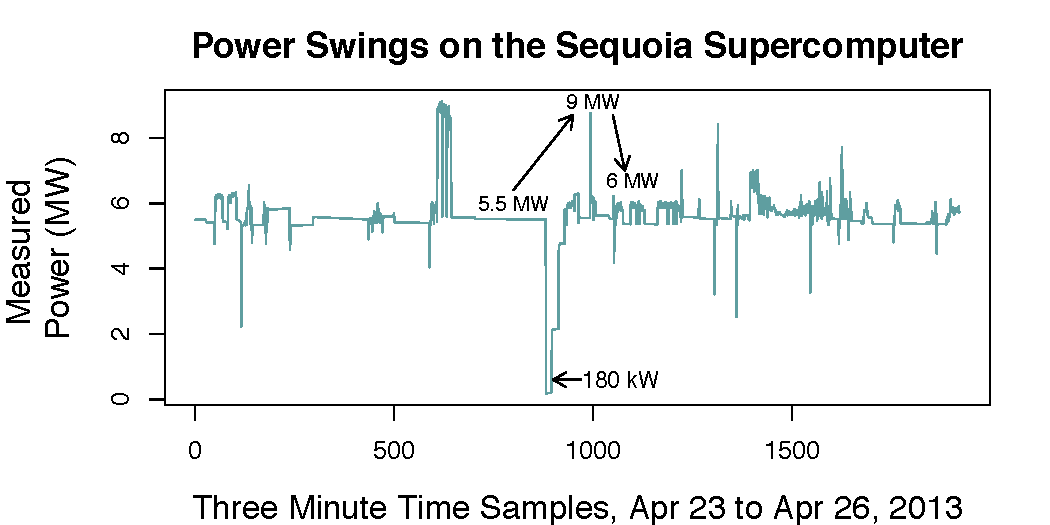
\includegraphics[scale=0.6]{figs/seq.pdf}}
\caption{Sequoia Supercomputer Power Swings}
\label{fig:seq}
\end{center}
\end{figure}

In our previous work, we focused on understanding how ESPs and SCs can work together to improve energy efficiency by surveying large-scale SCs in the United States \cite{BatesESP}. We developed a questionnaire and noted that none of the SCs are working directly with their ESPs. Our main conclusion from this work was that SCs in the United States were interested in a tighter integration with their ESPs, but a business case for the same had not been demonstrated. In this work, we expand our analysis to include European SCs, where electricity is more expensive and is subject to more variability because of the use of renewable sources of energy. We expected that the European SCs would be more tightly integrated with their ESPs because of the higher prices and more extensive use of renewables in Europe.  Contrary to our expectations, however, we found that the United States shows more interest in responding to requests from their ESPs than Europe.  There are four 10+MW SCs in the United States, whereas all of the remaining SCs in both the United States and Europe are 5MW or less.  These four 10+MW SCs have all had communication with their ESPs about responding to grid requests.  Perhaps they are harbingers for the lower power demand SCs.  Another factor explaining the difference may be greater availability of electricity demand response incentive programs in the United States than in Europe. In future studies, we hope to better understand the European ESPs and their environment to see if this hypothesis has merit. 

We accomplished expanding our analysis to Europe by extending the aforementioned questionnaire to European SCs. Nine out of the sixteen SCs that we contacted responded to the questionnaire. All except one of these sites were in Top 50 supercomputers in the world \cite{Top500}. Section \ref{res} presents an overview of our results from the questionnaire. Section \ref{spm} discusses the strategies, programs and methods that were used in the questionnaire and the willingness of respondents to consider these options. Section \ref{comm} highlights some of the comments we received from our respondents, and Section \ref{summary} concludes this article.

\section{Results: Europe and United States}
\label{res}
We noted that none of the European SCs communicated about grid integration and demand response techniques with their associated ESPs. Additionally, there was little interest in a tighter integration with the ESPs.

Figures \ref{fig:USload} and \ref{fig:EUload} depict the total load in megawatts for each of the respondents in the United States and in Europe. Most supercomputing sites have a total load of under 5 MW (sixteen out of twenty). Four of the surveyed supercomputing sites had a total load of over 10 MW. 
\begin{figure}
\begin{center}
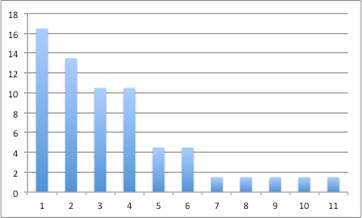
\includegraphics[scale=0.7]{figs/USLoad.jpg}
\caption{Total Load at at SCs in United States}
\label{fig:USload}
\end{center}
\end{figure}

\begin{figure}
\begin{center}
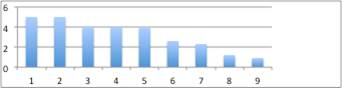
\includegraphics[scale=1]{figs/EULoad.jpg}
\caption{Total Load at at SCs in Europe}
\label{fig:EUload}
\end{center}
\end{figure}

Both United States and Europe had power swings and fluctuations of a few megawatts. In our questionnaire, we asked respondents to report the maximum variability that they have experienced in their SCs. The results of these for United States as well as Europe are shown in Figures \ref{fig:USvar} and \ref{fig:EUvar} respectively. In the United States, three of the eleven sites surveyed had maximum variability of over 5 MW. For our United States respondents, the minimal option for reporting this was ``Less than 3 MW'', because of which we could not capture less intense power swings. In the European survey, we allowed the respondents to provide a more accurate value, and as shown in Figure \ref{fig:EUvar}, we observed power swings in the range of half a megawatt to about 2 MW. Almost all of the respondents reported that this variability is due to maintenance cycles, and that it can be scheduled \emph{day-ahead} if necessary.

\begin{figure}
\begin{center}
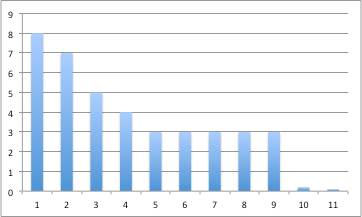
\includegraphics[scale=0.8]{figs/USVar.jpg}
\caption{Maximum Variability at at SCs in United States}
\label{fig:USvar}
\end{center}
\end{figure}

\begin{figure}
\begin{center}
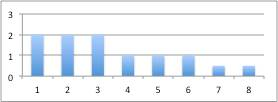
\includegraphics[scale=0.8]{figs/EUVar.jpg}
\caption{Maximum Variability at at SCs in Europe}
\label{fig:EUvar}
\end{center}
\end{figure}


\section{Strategies, Programs and Methods}
\label{spm}
In this subsection, we present the results of communication between SCs and their ESPs and the feasibility of a tighter integration. We define \emph{strategies} as power management techniques used by SCs to manage power. Strategies may or may not improve energy efficiency. For example, \emph{Load Migration} is a strategy that SCs may use in response to an ESP's request, and while it helps manage power effectively, it does not impact the energy efficiency of the site. On the other hand, fine-grained power management techniques, such as using node-level power capping, or better job scheduling algorithms are likely to improve energy efficiency but may not be as useful in response to an ESP request. Almost all sites employ some power management strategies, especially the ones involving lighting, temperature, cooling, fine-grain power management and job scheduling. There is moderate interest in grid integration strategies in the United States, and low interest in the same in Europe. From the point of view of SCs, strategies such as cutting jobs or load migration have little interest. 

\emph{Programs} are incentives offered by ESPs to their customers and to SCs in order to motivate them to help balance the electrical grid. Common examples include peak shedding, peak shifting and dynamic pricing. From our questionnaire, we concluded that neither European nor the United States sites are engaged with peak shedding, peak shifting or dynamic pricing programs at present. More sites in the United States have communicated with their ESPs regarding these programs. While both European and United States SCs are interested in dynamic pricing, there is mixed interest in peak shedding and peak shifting. The European sites are more interested in peak shedding than peak shifting, but the United States sites are more interested in peak shifting. 

We also asked our European respondents to indicate what might motivate them to communicate with their ESPs. The results are shown in Table \ref{fig:table2}. As can be noted from this figure, the main motivators are the financial incentives and the desire to be ``good citizens.''

\begin{figure}
\begin{center}
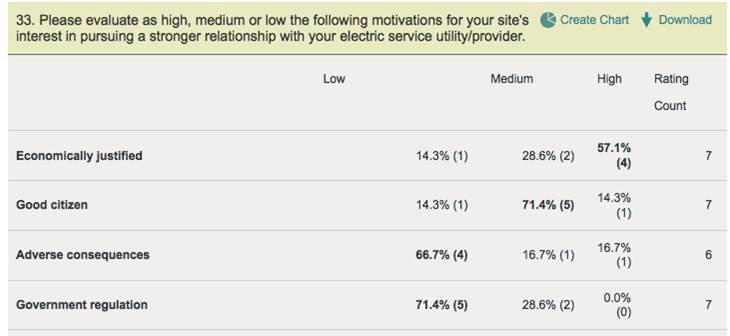
\includegraphics[scale=0.5]{figs/Table2.jpg}
\caption{Motivation}
\label{fig:table2}
\end{center}
\end{figure}

\emph{Methods} are used by the ESPs to balance the electrical grid in the transmission and distribution phases. Examples of methods include regulation, frequency response, grid scale storage and use of renewable sources of energy. Both European and US sites are interested in discussing renewables with their ESPs, but there is little interest in communicating with regards to the other possible methods.

\section{Comments}
\label{comm}
From the comments section in our questionnaire, we noted that all SCs are already using \emph{demand forecasting} to communicate their upcoming demands and maintenance cycle schedules with their ESPs. For example, one comment was ``We project hourly average power at least a day in advance, within +/- 1MW''. Another interesting comment was ``We've to ensure that our power load neither over- nor undershoots the contracted power band. In any cases of foreseen power abnormalities we've to inform our grid provider at least two days ahead of schedule.''

One of the SCs mentioned that they could not provide the forecast that was being asked by their ESP. More specifically, their comment indicated that their ESP asked for ``multi-year forecast of energy requirements, additional detailed forecasting and ultimately real time data, and power projections, hour by hour, for at least a day in advance.''

When it came to ESP programs, the United States SCs showed more interest. ``Our site generates 30-35 MW of power yet still imports 5-10 MW. As a large generation source the utility providers see the campus as a highly attractive partner for offloading grid stress. automatic load shedding is being explored/deployed today, '' one of the SCs noted. Another comment was ``[We are] working on load sharing of data with utility to provide better scheduling tools and address potential grid changes.'' One of the SCs mentioned that they demonstrated that peak shedding and shifting was possible, but not deployed due to its impact on HPC productivity. 

The European SCs, on the other had, did not have much knowledge about ESP programs. Some of the responses were ``There are not so many related options and features offered by providers. We are open to further and pro-active efforts as long as providers have other kinds of programs to propose'' and ``With many of your questions I am wondering about the kind of contracts other centers might have and about the quality of some electricity providers.''

The comments also indicated that the SCs in United States are investigating the impact of power fluctuations on the electrical grid. ``[We are] working directly with provider to ensure that the effects of large load swings are understood. Have funded a simulation that accounts for all loads.'' and ``Our provider has no problem with our load swings. They indicate no concern with our next system either, but we are still looking into possible options in case there actually is a problem.'' were some of the interesting responses.

\section{Summary and Next Steps}
\label{summary}

\begin{figure}
\begin{center}
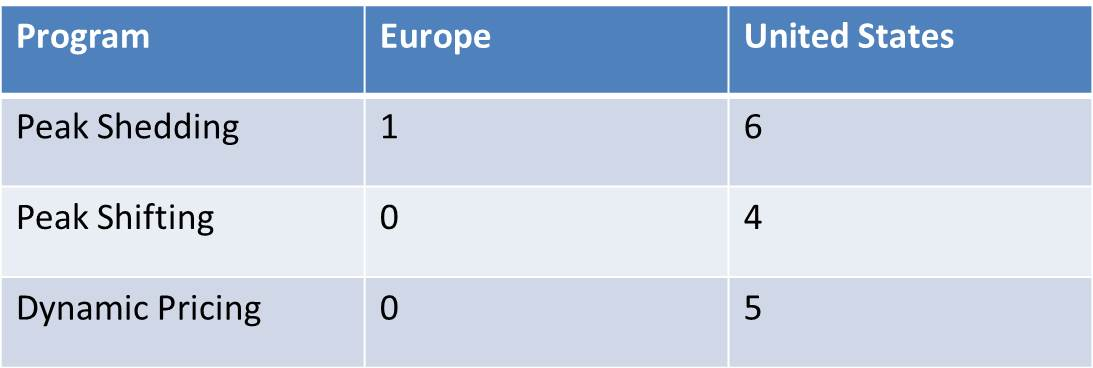
\includegraphics[scale=0.5]{figs/Table3.jpg}
\caption{Communications with ESPs regarding available programs}
\label{fig:table3}
\end{center}
\end{figure}

In summary, we believe that the European ESP programs need to be studied in greater detail, and awareness regarding these programs needs to be raised among the SCs. In general, the SCs in the United States seem to have a closer relationship with their ESPs than the ones in Europe. This can also be verified from Table \ref{fig:table3}, which shows that only 1 of the 9 respondents in Europe has had a discussion about programs with their ESP. As part of our future work, we want to explore the European ESP programs further, and also conduct a similar study in Japan.

\bibliographystyle{plain}
\bibliography{refs}
\end{document}
